% Created 2021-12-15 Wed 15:05
\documentclass[9pt, b5paper]{article}
\usepackage[UTF8]{ctex}
\usepackage{xltxtra}
\usepackage{bera}
\usepackage[T1]{fontenc}
\usepackage[scaled]{beraserif}
\usepackage[scaled]{berasans}
\usepackage[scaled]{beramono}
\usepackage{graphicx}
\usepackage{xcolor}
\usepackage{multirow}
\usepackage{multicol}
\usepackage{float}
\usepackage{textcomp}
\usepackage{geometry}
\geometry{left=1.2cm,right=1.2cm,top=1.5cm,bottom=1.2cm}
\usepackage{algorithm}
\usepackage{algorithmic}
\usepackage{latexsym}
\usepackage{natbib}
\usepackage{minted}
\newminted{common-lisp}{fontsize=ootnotesize}
\usepackage[xetex,colorlinks=true,CJKbookmarks=true,linkcolor=blue,urlcolor=blue,menucolor=blue]{hyperref}
\author{deepwaterooo}
\date{\today}
\title{NDK 高级编程(笔记)}
\hypersetup{
  pdfkeywords={},
  pdfsubject={},
  pdfcreator={Emacs 27.1 (Org mode 8.2.7c)}}
\begin{document}

\maketitle
\tableofcontents


\section{深入了解 Android NDK}
\label{sec-1}
\begin{itemize}
\item 本文链接:\url{http://gnaixx.cc/2017/07/23/20170723-ndk-pro/}
\item 创建项目时 Android.mk 文件的构建:Android.mk配置参数
\item ndk-build 脚本参数
\begin{minted}[frame=lines,fontsize=\scriptsize,linenos=false]{shell}
#NDK 项目位置
ndk-build -C /path/to/the/project
#强制重构所有代码
ndk-build -B
#清除生成的二进制文件和目标文件
ndk-build clean
#并行构建命令
ndk-build -j 4
\end{minted}
\end{itemize}

\section{用 JNI 实现与原生代码通信}
\label{sec-2}
jni 的开发基础知识,参考:
\begin{itemize}
\item NDK开发 - JNI开发流程
\item NDK开发 - JNI数据类型与Java数据类型映射关系
\item NDK开发 - JNI基本数据和字符串处理
\item NDK开发 - JNI数组数据处理
\item NDK开发 - C/C++ 访问 Java 变量和方法
\item NDK开发-JNI 局部引用、全局引用和弱全局引用
\end{itemize}

\section{日志、调试及故障处理}
\label{sec-3}
\subsection{原生日志 API}
\label{sec-3-1}
\begin{minted}[frame=lines,fontsize=\scriptsize,linenos=false]{shell}
//头文件
#include <android.h>
//Android.mk
LOCAL_LALIBS += -llog
_android_log_write(ANDROID_LOG_DEBUG, "hello-jni", "debug log.")
//多参数封装
static void logMessage(JNIEnv *env, jobject obj, const char *format, ...) {
    static jmethodID methodID = NULL;
    if (NULL == methodID) {
        jclass clazz = env->GetObjectClass(obj);
        methodID = env->GetMethodID(clazz, "logMessage", "(Ljava/lang/String;)V");
        env->DeleteLocalRef(clazz);
    }
    if(methodID != NULL) {
        char buffer[MAX_LOG_MSG_LENGTH];
        va_list ap;
        va_start(ap, format); //指向 format 后可变参数的地址
        vsnprintf(buffer, MAX_LOG_MSG_LENGTH, format, ap);
        va_end(ap);
        jstring message = env->NewStringUTF(buffer);
        if (message != NULL) {
            env->CallVoidMethod(obj, methodID, message);
            env->DeleteLocalRef(message);
        }
    }
}
\end{minted}

\subsection{重定向 Android 日志}
\label{sec-3-2}
\begin{minted}[frame=lines,fontsize=\scriptsize,linenos=false]{shell}
adb shell stop
adb shell setprop log.redirect-stdio true
adb shell start
\end{minted}

\subsection{故障处理}
\label{sec-3-3}
\subsubsection{堆栈分析}
\label{sec-3-3-1}
\begin{minted}[frame=lines,fontsize=\scriptsize,linenos=false]{shell}
#ndk-stack
adb logcat | ndk-stack -sym obj/local/armeabi
#arm-linux-androideabi-addr2line
arm-linux-androideabi-addr2line -e obj/local/armeabi-v7a/libtongdun.so 0002197e
\end{minted}
\subsubsection{启用 CheckJNI:}
\label{sec-3-3-2}
\begin{minted}[frame=lines,fontsize=\scriptsize,linenos=false]{shell}
adb shell setprop debug.checkjni 1
\end{minted}
\subsection{内存问题}
\label{sec-3-4}
\subsubsection{打开 libc 调试模式}
\label{sec-3-4-1}
\begin{minted}[frame=lines,fontsize=\scriptsize,linenos=false]{shell}
adb shell setprop libc.debug.malloc 1
adb shell stop
adb shell start
\end{minted}
\subsubsection{strace 工具}
\label{sec-3-4-2}
\begin{minted}[frame=lines,fontsize=\scriptsize,linenos=false]{shell}
#获取进程
adb shell ps | grep packagename
#附加进程
adb shell strace -v -p <pid>
\end{minted}

\section{原生线程}
\label{sec-4}
\begin{itemize}
\item 源码地址: ndk-pro/threads
\begin{itemize}
\item \url{https://github.com/gnaixx/pro-ndk/tree/master/threads}
\end{itemize}
\end{itemize}
\subsection{POSIX 线程返回结果}
\label{sec-4-1}

//1.线程句柄 2.返回值指针
int pthread\_join(pthread\_t thread, void** ret\_val);
\subsection{POSIX 线程同步}
\label{sec-4-2}
\begin{minted}[frame=lines,fontsize=\scriptsize,linenos=false]{shell}
static pthread_mutex_t mutex;
//初始化
int pthread_mutex_init(pthread_mutex_t* mutex, const pthread_mutexarrt_t* attr);
//锁定
int pthread_mutex_lock(pthread_mutex_t* mutex);
//解锁
int pthread_mutex_unlock(pthread_mutex_t* mutex);
//销毁
int pthread_mutex_destroy(pthread_mutex_t* mutex);
\end{minted}
\subsection{使用信号量同步 POSIX 线程}
\label{sec-4-3}
\begin{minted}[frame=lines,fontsize=\scriptsize,linenos=false]{shell}
//头文件
#include <semaphone.h>
//初始化
extern int sem_init(sem_t* sem, int pshared, unsigned int value);
//锁定信号
extern int sem_wait(sem_t* sem);
//解锁
extern int sem_post(sem_t* sem);
//销毁
extern int sem_destroy(sem_t* sem);
\end{minted}

\section{POSIX Socket API}
\label{sec-5}
\begin{itemize}
\item TCP \&\& UDP
\item 源码地址: pro-ndk/echo
\begin{itemize}
\item \url{https://github.com/gnaixx/pro-ndk/tree/master/echo}
\end{itemize}
\end{itemize}

\section{支持 C++}
\label{sec-6}
\subsection{支持的 C++ 运行库}
\label{sec-6-1}
\begin{itemize}
\item C++系统运行库 不支持:C++标准库、 异常支持库、 RTTI 支持
\item GAbi++、 STLport、 GUN STL

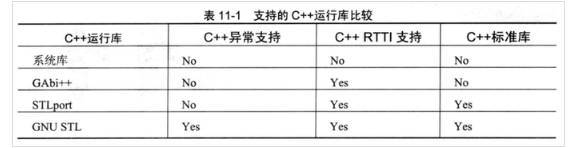
\includegraphics[width=.9\linewidth]{./pic/stl.png}
\end{itemize}
\subsection{指定 C++ 运行库}
\label{sec-6-2}
\begin{minted}[frame=lines,fontsize=\scriptsize,linenos=false]{shell}
//Application.mk
APP_STL := system //默认
APP_STL := gabi++_static
APP_STL := gabi++_shared
APP_STL := stlport_static
APP_STL := stlport_shared
APP_STL := gunstl_static
APP_STL := gunstl_shared
//1.项目只有一个单一的原生模块时支持静态库
//2.项目中包含多个原生模块时使用动态库
//3.动态库使用时需要先加载 
System.loadLibrary(“strport_shared”)
\end{minted}
\subsection{C++支持异常}
\label{sec-6-3}
\begin{minted}[frame=lines,fontsize=\scriptsize,linenos=false]{shell}
//单个模块 Android.mk
LOCAL_CPP_FEATURES += exceptions
//支持所有原生模块 Application.mk
APP_CPPFLAGS += -fexceptions
\end{minted}
\subsection{C++ RTTI 支持(Run-Time Type Information)}
\label{sec-6-4}
\begin{itemize}
\item 在运行库展示对象类型信息,只要用于执行安全类型转化。
\begin{minted}[frame=lines,fontsize=\scriptsize,linenos=false]{shell}
//单个模块 Android.mk
LOCAL_CPP_FEATURES += rtti
//支持所有原生模块 Application.mk
APP_CPPFLAGS += -frtti
\end{minted}
\end{itemize}
\subsection{C++ 标准库}
\label{sec-6-5}

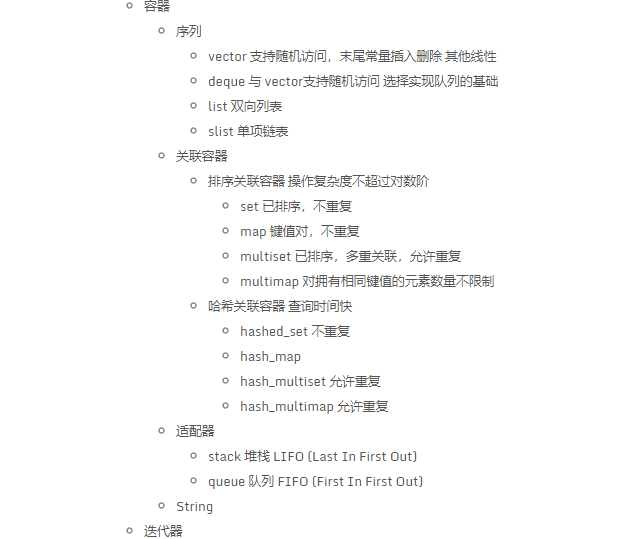
\includegraphics[width=.9\linewidth]{./pic/c++stdlib.png}
\subsection{C++ 运行库调试模式}
\label{sec-6-6}
\begin{minted}[frame=lines,fontsize=\scriptsize,linenos=false]{shell}
//GUN STL 调试模式
LOCAL_CFLAGS += -D_GLIBCXX_DEBUG
//STLport 调试模式
LOCAL_CFLAGS += -D_STLP_DEBUG
//日志重定向到 Android 日志 
LOCAL_CFLAGS += -D_STLP_DEBUG
LOCAL_CFLAGS += -D_STLP_DEBUG_MESSAGE
LOCAL_LDLIBS += —llog
void __stl_debug_message(const char* format_str, …){
    va_list ap;
    va_start(ap, format_str);
    __android_log_vprint(ANDROID_LOG_FATAL, “STLport”, format_str, ap);
    va_end(ap);
}
\end{minted}
\section{原生图形 API}
\label{sec-7}
\begin{itemize}
\item 源码地址: ndk-pro/abiplayer
\begin{itemize}
\item \url{https://github.com/gnaixx/pro-ndk/tree/master/aviplayer}
\end{itemize}
\end{itemize}
\section{程序概要分析和 NEON 优化}
\label{sec-8}
\begin{itemize}
\item android-ndk-profiler
\item NEON 指令:并不是所有基于 ARM-V7a 的设备都支持 NEON 指令
\end{itemize}
% Emacs 27.1 (Org mode 8.2.7c)
\end{document}